\iffalse
\begin{figure}[htbp]
\centering
\begin{subfigure}[t]{0.40\textwidth}
	\centering
	\resizebox{\linewidth}{!}{
	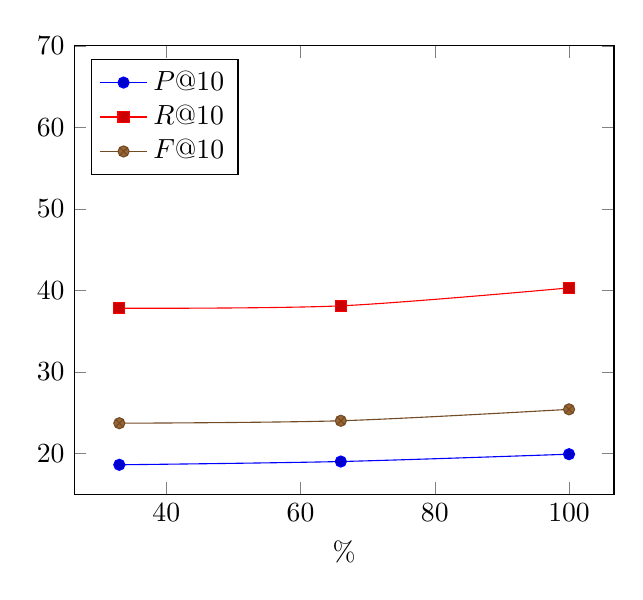
\begin{tikzpicture}%[font=\huge]
	\begin{axis}[smooth, xlabel={$\%$}, %ylabel={$\%$},
				 ymin=15, ymax=70, legend pos=north west]

		\addplot+ coordinates{(33, 18.6)(66, 19.0)(100, 19.9)};
		\addlegendentry{$P@10$}
		\addplot+ coordinates{(33, 37.8)(66, 38.1)(100, 40.3)};
		\addlegendentry{$R@10$}
		\addplot+ coordinates{(33, 23.7)(66, 24.0)(100, 25.4)};
		\addlegendentry{$F@10$}

		%\addplot+[mark=triangle*] coordinates{(33, 26.5)(66, 26.8)(100, 28.2)}; %\addlegendentry{P\@5}
		%\addplot+[mark=*] coordinates{(33, 27.9)(66, 27.8)(100, 29.6)}; %\addlegendentry{R\@5}
		%\addplot+[mark=square*] coordinates{(33, 26.0)(66, 26.0)(100, 27.6)}; %\addlegendentry{F\@5}
	\end{axis}
	\end{tikzpicture}
	}
	\caption{KP20k}
\end{subfigure}
%
\begin{subfigure}[t]{0.40\textwidth}
	\centering
	\resizebox{\linewidth}{!}{
	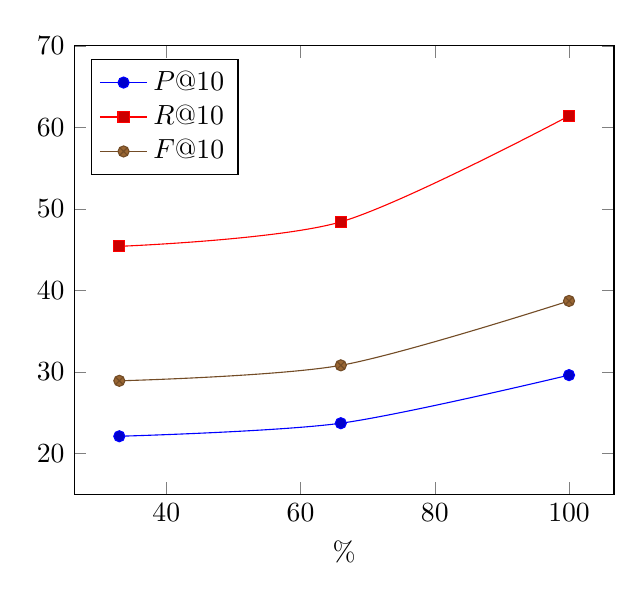
\begin{tikzpicture}%[font=\huge]
		\begin{axis}[
		    smooth,
		    xlabel={$\%$}, %ylabel={$\%$},
	    	ymin=15, ymax=70,
			legend pos=north west
		]

		\addlegendentry{$P@10$}
		\addplot coordinates{(33, 22.1)(66, 23.7)(100, 29.6)};
		
		\addlegendentry{$R@10$}
		\addplot coordinates{(33, 45.4)(66, 48.4)(100,61.4)};
		
		\addlegendentry{$F@10$}
		\addplot coordinates{(33, 28.9)(66, 30.8)(100, 38.7)};
		
		%\addplot+[smooth] coordinates{(33, 33.8)(100, 46.3)}; %\addlegendentry{P\@5}
		%\addplot+[smooth] coordinates{(33, 35.2)(100, 49.3)}; %\addlegendentry{R\@5}
		%\addplot+[smooth] coordinates{(33, 33.3)(100, 46.0)}; %\addlegendentry{F\@5}
		\end{axis}
	\end{tikzpicture}
	}
	\caption{KPTimes}
\end{subfigure}
    \vspace{-1em}
	\caption{Performances de CopyRNN en fonction de la taille du jeu de donnée d'entraînement.} \label{fig:train_percent}
\end{figure}
\fi

\begin{figure}
	\centering
	%\resizebox{.9\textwidth}{!}{
	\begin{tikzpicture}%[font=\huge]
	\begin{axis}[
	    scaled x ticks=false,
	    smooth, xlabel={$\#$ documents}, ylabel={$\%$ F@10},
		ymin=21, ymax=44,
		%legend pos=north east,
		legend pos=outer north east,
		xmin=0, xmax=600000,
		%xticklabels={0,100\,K,200\,K,300\,K,400\,K,500\,K},
        %xtick = {0,100000,200000,300000,400000,500000}]
        xticklabels={100\,K,300\,K,500\,K},
        xtick = {100000,300000,500000},
        ]

        \addplot+[color2,every mark/.append style={color=white,fill=color2},mark=*] coordinates{(86641, 34.4)(173282, 37.6)(259923, 38.7)};
        \addlegendentry{NYTimes}


        \addplot[color1,every mark/.append style={color=white,fill=color1},mark=X*] coordinates{(175696, 23.7)(351393, 24.0)(527090, 25.4)};
		\addlegendentry{KP20k}
	\end{axis}
	%https://tex.stackexchange.com/questions/413237/get-legend-outside-plot-on-tikz-and-customise-axis-labels
	%https://tex.stackexchange.com/questions/278530/how-i-can-customize-a-legend-on-pgfplots
	\iffalse
	\matrix [draw, matrix of nodes,
            anchor=south east,
        ] at (legend) {
        \multicolumn{2}{c}{Métrique} \\
        \ref{pgfplots:c2r1} & $P@10$ \\
        \ref{pgfplots:c2r2} & $R@10$ \\
        \ref{pgfplots:c2r3} & $F@10$ \\
        \multicolumn{2}{c}{Corpus} \\
        \ref{pgfplots:c2r2} & KP20k \\
        \ref{pgfplots:c2r2} & KPTimes \\
    };
	\fi
	%}
	\end{tikzpicture}
	\caption{Performances de CopyRNN (F@10) en fonction de la taille du jeu de données d'entraînement.}
	\label{fig:train_percent}
\end{figure}
